\newcommand{\CLASSINPUTtoptextmargin}{2cm}
\newcommand{\CLASSINPUTbottomtextmargin}{1in}
\documentclass[journal, a4paper]{IEEEtran}

\usepackage{graphicx}
\usepackage{url}
\usepackage{amsmath}
\usepackage{url}
\usepackage[hyperfootnotes=false]{hyperref}
\usepackage[scientific-notation=true]{siunitx}
\usepackage{subcaption}
\usepackage{setspace}
\usepackage{vector}
\usepackage{amssymb}
\usepackage{tgtermes}
\usepackage{gensymb}
\usepackage{multirow}
\usepackage[
singlelinecheck=false % <-- important
]{caption}
\usepackage{datetime}



\DeclareGraphicsExtensions{.pdf,.png,.jpg}


\usepackage{epstopdf}

% Your document starts here!
\begin{document}
% Define document title and author
\title{\huge Calibration of the High Momentum Spectrometer Drift Chambers}
\author{Carlos Yero\\March 20, 2017}
\maketitle
\vspace{1mm}
% Write abstract here
\begin{abstract}
The calibration procedure for \textit{horizontal} drift chambers in the High Momentum Spectrometer (HMS) is outlined. The main
objective of this calibration was to produce a time-to-distance map in order to determine the position of
particle tracks from the measured drift times. Using the calibration results, a brief study about drift velocities was
also done in which it was found that they vary from $\sim$ 40-55$\mu$m/ns in regions of approximately uniform electric fields.
Finally, efficiency and residuals on both chambers was investigated and determined each plane to be better than
94\% efficient, with spatial resolutions better than 420 $\mu$m.
\end{abstract}
\section{Introduction}
% \PARstart{}{} creates a tall first letter for this first paragraph
\PARstart{A}{s} part of the plan to commission the Super HMS (SHMS) at Hall C - Jefferson Lab, the
HMS also needs to be operational for coincidence experiments. The drift chambers are an essential element
of the spectrometer as they are needed for particle tracking and reconstruction. (See Figure \ref{fig:HMS_carriage}) One of the drift chambers
in the HMS had 97 sense wires and 1 field wire damaged from years of exposure to radiation since it was first
installed in the detector stack in 1995 \cite{baker}. The  wires were replaced on Fall 2016 and both chambers
were verified to be operational by performing several cosmic\footnote{Cosmic tests refers to the detection of cosmic rays or highly energetic particles (mainly
protons) originating mostly outside of the solar system.} tests. On March 2017, as part of the Key Performance Parameters (KPP)
neede to be satisfy by Hall C to demonstrate that the SHMS was in operating conditions, data was taken with actual beam in the
Hall. Data with the HMS was also taken and used to calibrate the drift chambers.
\begin{figure}[h]
  \centering
  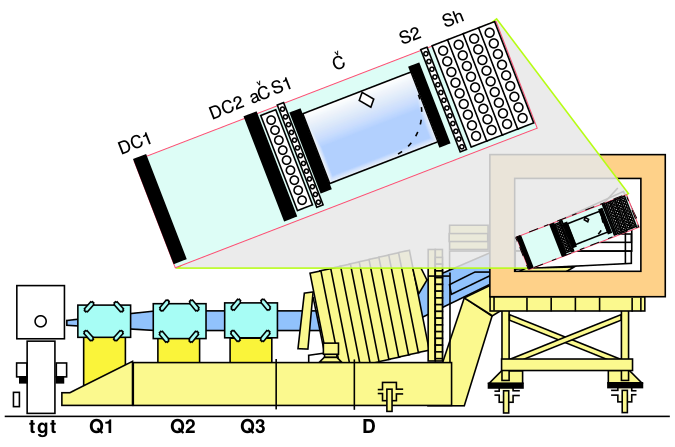
\includegraphics[width=2.8in, height=1.8in]{HMS_Carriage.png}
  \caption{HMS carriage showing the magnet elements (Quadrupoles ($Q_{i}$), Dipole (D)). The detector elements are
  after the 25$^{\circ}$ bend, where DC1 and DC2 denotes the drift chamber
  packages 1 and 2.}
  \label{fig:HMS_carriage}
\end{figure}
% Main Part
\section{Principle of Operation}
Each drift chamber consists of 6 planes (X, Y, U, V, Y', X'), where the X(X') are orthogonal to Y(Y') planes, and U and V are
tilted 15\degree  relative to X(X'). (See Figure \ref{fig:wireplanes})
\begin{figure}[h]
  \centering
  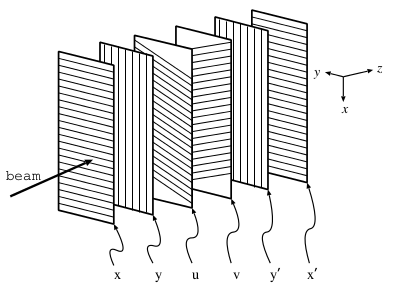
\includegraphics[width=2.8in, height=1.8in]{wire_planes.png}
  \caption{Schematic of drift chamber planes. Figure courtesy of C. Armstrong.}
  \label{fig:wireplanes}
\end{figure}
Each plane consists of an array of alternaring field and sense wires\footnote{Total sense wires per plane: X,X'-113, Y,Y'-52, U,V-107} (0.5 cm apart) surrounded by
two arrays of field wires so that each sense wire is surrounded by 8 field wires, forming a cell. (See Figure \ref{fig:wire_cell})
\begin{figure}[h]
  \centering
  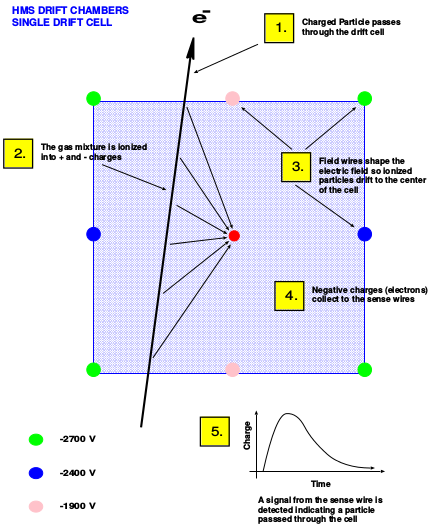
\includegraphics[width=3.0in, height=3.0in]{wire_cell.png}
  \caption{Schematics of a single cell in a drift chamber plane. Figure
  courtesy of G. Niculescu and D. Abbot.}
  \label{fig:wire_cell}
\end{figure}
The field wires are kept at a negative potential while the sense wires are grounded (0 V). Due to
the potential difference between the field and sense wires, an electric field is established which causes
free electrons from ionized gas atoms and molecules of
the gas mixture\footnote{Drift chambers are filled with a gas mixture mainly to make the ions drift velocity
as uniform as possible.} to drift towards the sense wires producing a measurable signal.
The sense wire signals are pre-amplified and read by 16-channel input discriminators which produce logic signals that lead into Time-to-Digital
Converters (TDCs) by twisted pair ribbon cables\cite{meekins}. The TDCs registers the total travel time
of the signal since it was created by the passing particle. This time is compared to the surveyed time it would have taken the signal to propagate across
the sense wire, through the ribbon cable into the TDC if the particle would have passed through the sense wire. The time difference
is known as the \textit{drift time}, or the time it takes the free electrons to drift towards the sense wire.
 Mathematically, the drift time can be expressed as,
\begin{equation}
t_{D} = (t_{meas.}-t_{REF}) - [\underbrace{(t_{wire} + t_{cable})}_{t'} - t_{REF}]
\end{equation}
where $t_{meas.}$ is the measured time by the TDC, and $t'$ is the time it takes the signal to propagate
across the sense wire and through the cable into the TDC if the track would have passed through the sense wire. These times
are measured relative to a reference time\footnote{Reference time (trigger) is defined based on certain conditions that
a signal must pass for it to be considered as a physical event. In the HMS in particular, it was defined as a 3/4
hodoscope plane coincidence - or the signal must have been detected in at least 3/4 hodoscopoe planes within a
time window for it to be considered a true event (or trigger).} $t_{REF}$, used by the TDCs in Common Stop Mode (analogous to
a stopwatch). \\
\indent For a charged particle that traverses the drift chamber, only certain sense wires will fire.
If a wire, say in the X-plane fires, one does not know if the particle passed the left or right side of the chamber
relative to the wire. By including the X'-plane, the left-right ambiguity is removed since the particle will fire a wire in X' which
allows one to determine the x-coordinate of the track. Similarly, for the Y (Y') planes, the y-coordinate of the track is
determined and the U (V) planes provide angle information about the track.\\
\indent A coarse track reconstruction can be done with only the knowledge of the wires that fire from a physics
event. Knowing the associated drift times of the wires that were hit, however, allows for a more precise track reconstruction,
as the drift time can be converted to a drift distance from the determination of time to distance maps from calibration. The
drift distances can be added as fine corrections to the coarse track reconstruction.
\section{Calibration Procedure}
\noindent For many events illuminating all cells in any give plane, one obtains a drift time distribution
for each sense wire which are then averaged over the entire plane to form a drift time distribution per plane.(see Figure \ref{fig:hdc2y1_time})
\begin{figure}[!ht]
  \centering
  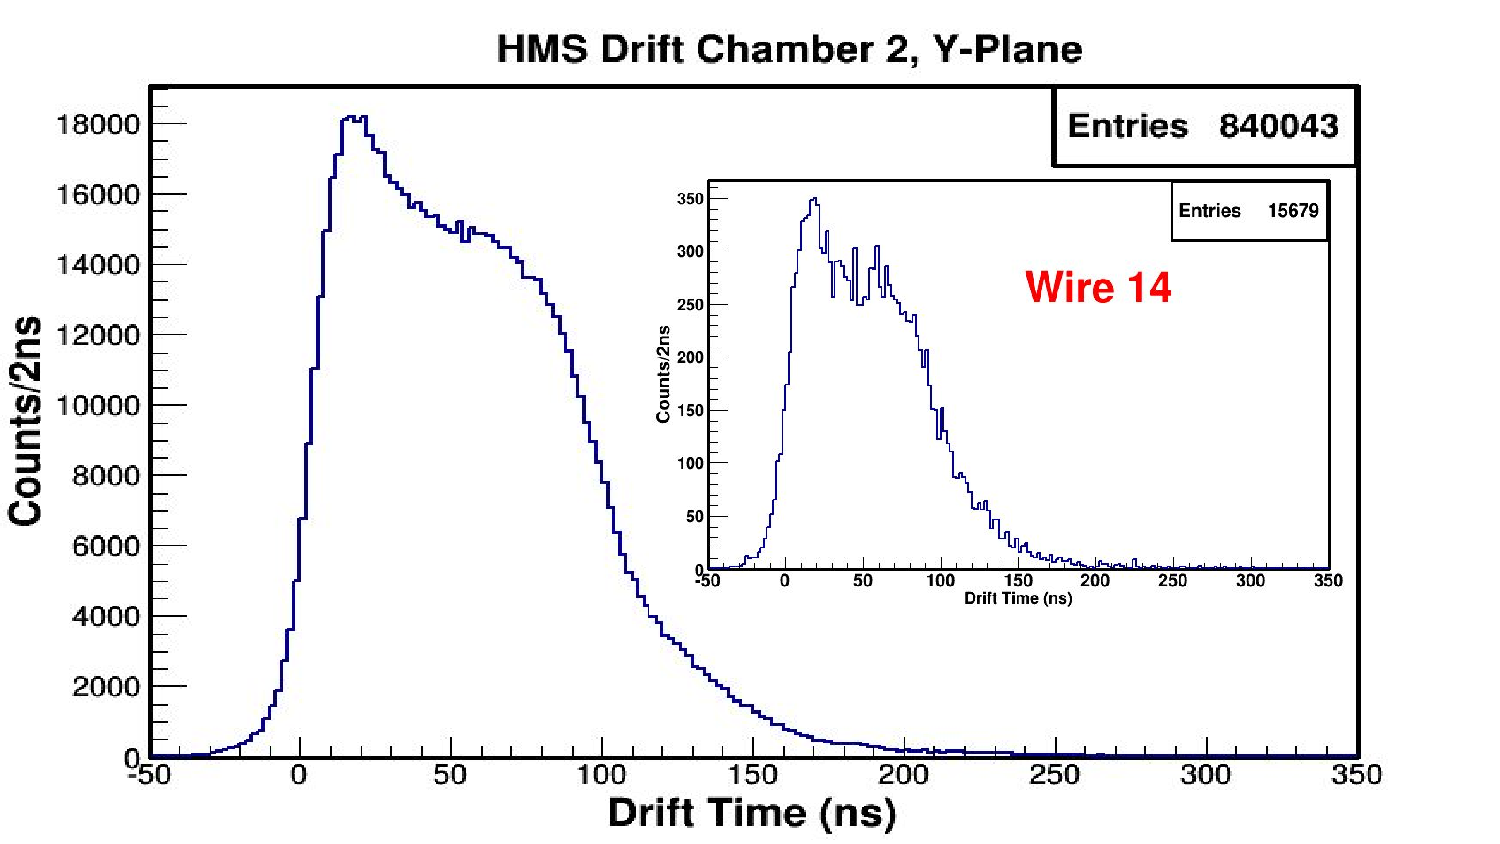
\includegraphics[width=3.8in, height=2.3in]{hdc2y1_time.pdf}
  \caption{Averaged and single wire drift time spectra in the Y-plane of drift chamber 2.}
  \label{fig:hdc2y1_time}
\end{figure}

Associated with each drift time spectra is a quantity called $``t_{0}"$. The $``t_{0}"$ corresponds to the
location in the histogram where the ionized particle comes in contact with the wire. If its value is anything other
than zero nanoseconds (0 ns), it is interpreted as the value by which the drift time must be shifted in order to
align the $``t_{0}"$ with 0 ns. All subsequent times in each drift time spectra are measured relative to this time.\\
\indent The $``t_{0}"$ for each plane is determined by calculating the $``t_{0}"$ for individual wires in each plane and taking a
weighted average. The $``t_{0}"$ for individual sense wires is determined by a linear fit of the wire drift time spectra at around 20\% of the peak
$\pm \Delta t$ for each sense wire, where $\Delta t$ is the fit range. The linear fit is then extrapolated to the
horizontal axis (drift time), and this extrapolated value is defined as $``t_{0}"$. (See Figure \ref{fig:wire_fit})
\begin{figure}[!ht]
  \centering
  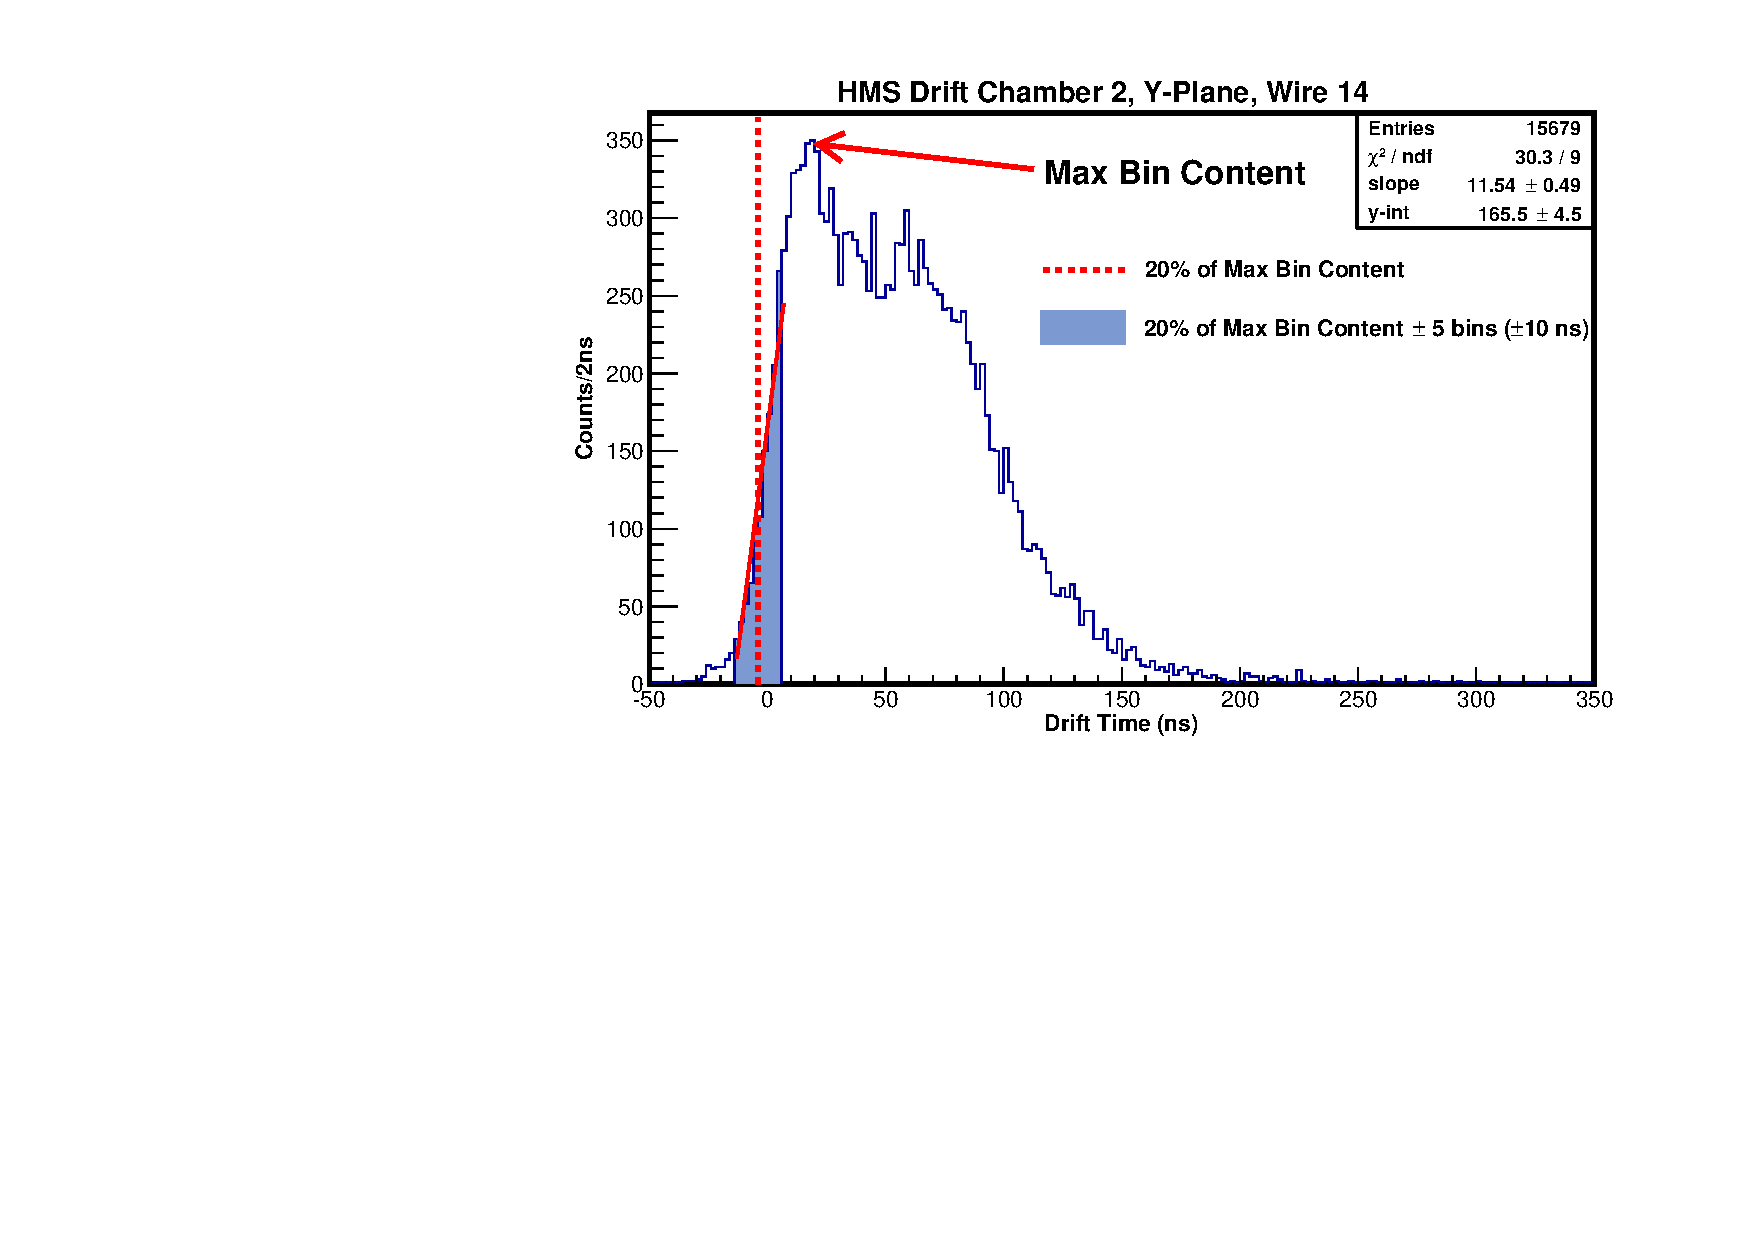
\includegraphics[width=3.8in, height=2.3in]{hdc2y1_w14_fit.pdf}
  \caption{Linear fit to drift time of sense wire 14 in the Y-plane of the second drift chamber. The fit is extrapolated to the
  x-axis to determine $``t_{0}"$. }
  \label{fig:wire_fit}
\end{figure} \\
Less than a percent of the total wires in the second drift chamber were found dead\footnote{Wires with no registered hits, except noise from the electronics, are defined as dead.}, while other wires had
low statistics due to the biased direction of the particles entering the detector stack. This effect can be observed
from the wire hitmaps in Figure \ref{fig:hdc2y1_hitmap}.
\begin{figure}[!ht]
  \centering
  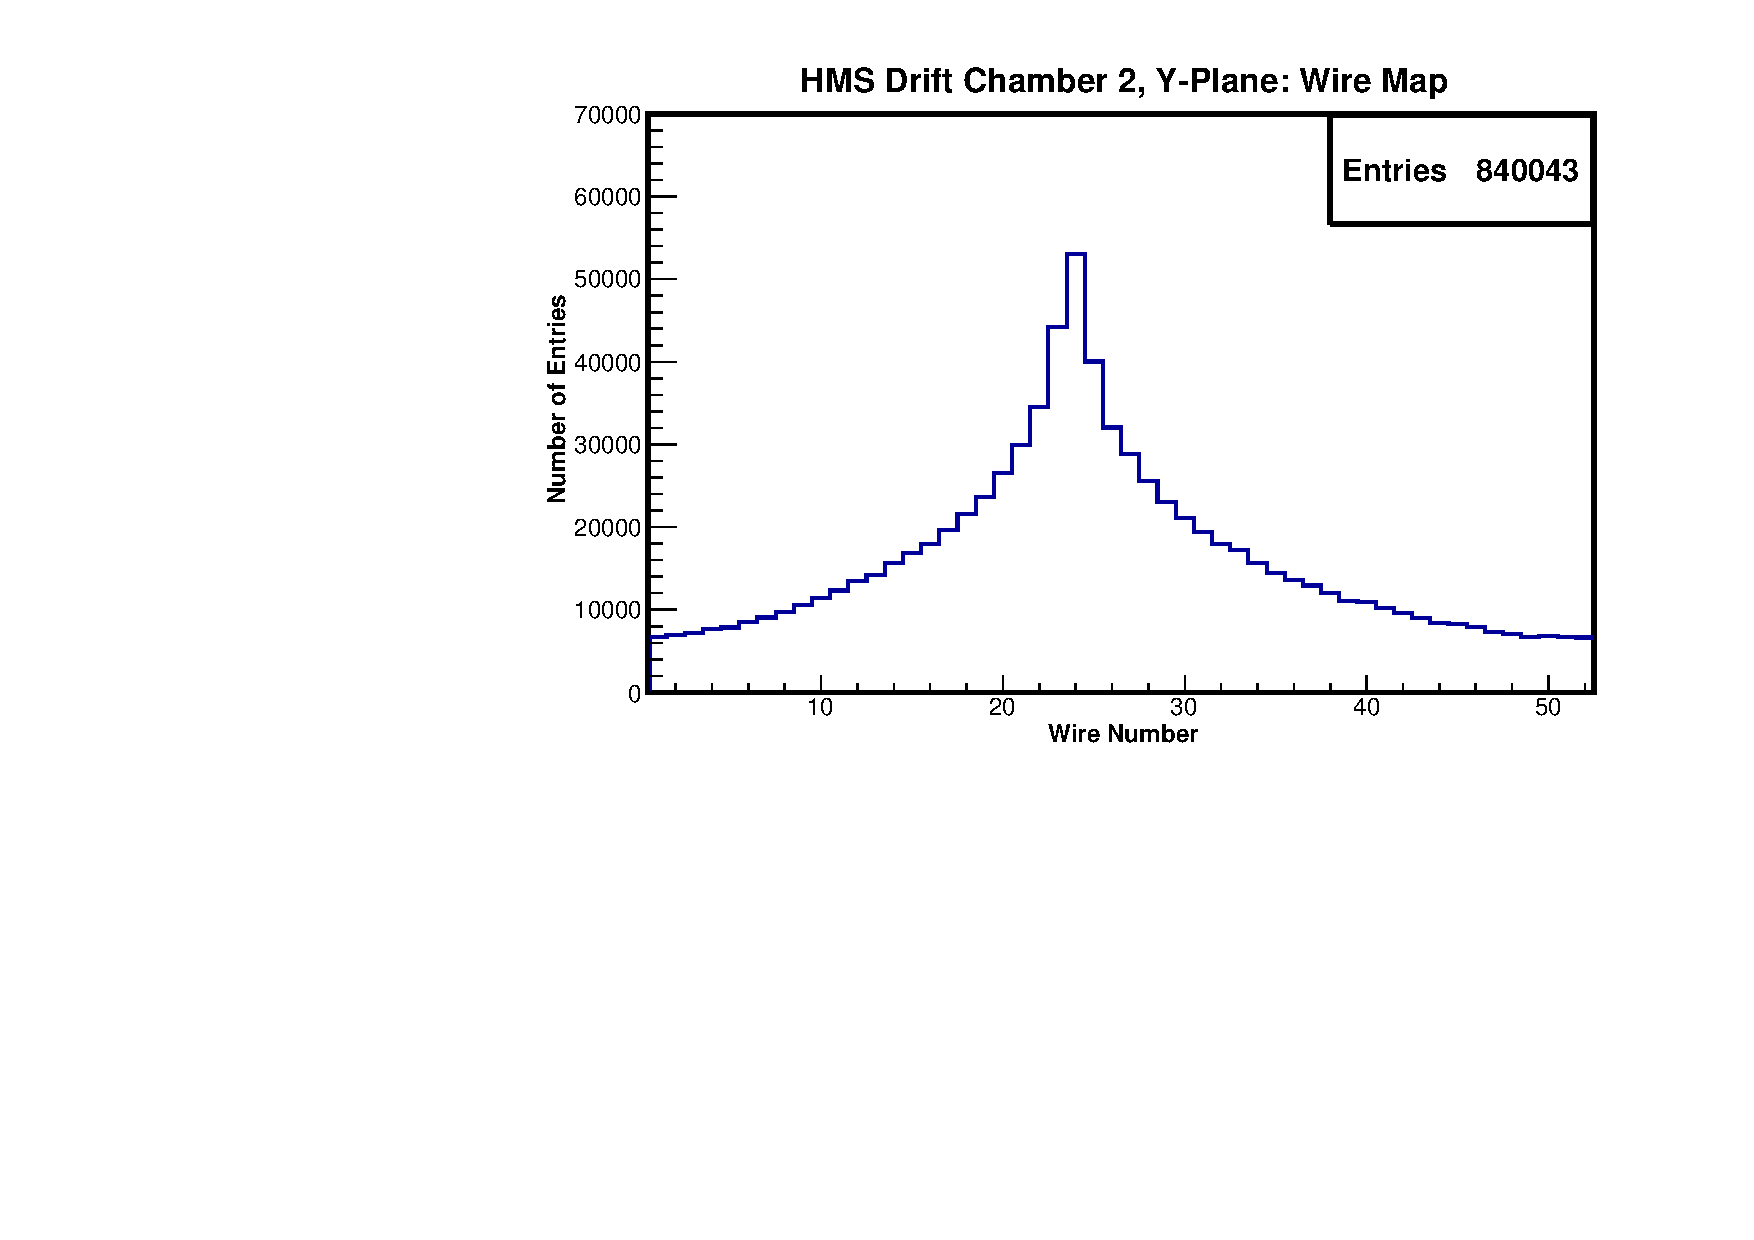
\includegraphics[width=3.8in, height=2.3in]{hdc2y1_wiremap.pdf}
  \caption{Wire map showing the number of entries (hits from physics events) received by each sense wire in Y-plane of
  the second drift chamber.}
  \label{fig:hdc2y1_hitmap}
\end{figure}
The central wire from the Y-plane has the highest number of entries and fall exponentially for wires further from the
center. This effect is due to the spectrometer magnets focusing the particles that enter the detector stack towards
the center (focal plane) of the two chambers.
The calibration run taken had enough statistics, that even at the edge wires had sufficient events for a linear
fit to be made. Dead wires found in other planes were excluded from the fit, as they would have been outliers in
the data, causing a shift in the weighted average. The weighted average for the Y-plane of drift chamber 2 is shown
in Figure \ref{fig:hdc2y1_wght_avg}.
\begin{figure}[!ht]
  \centering
  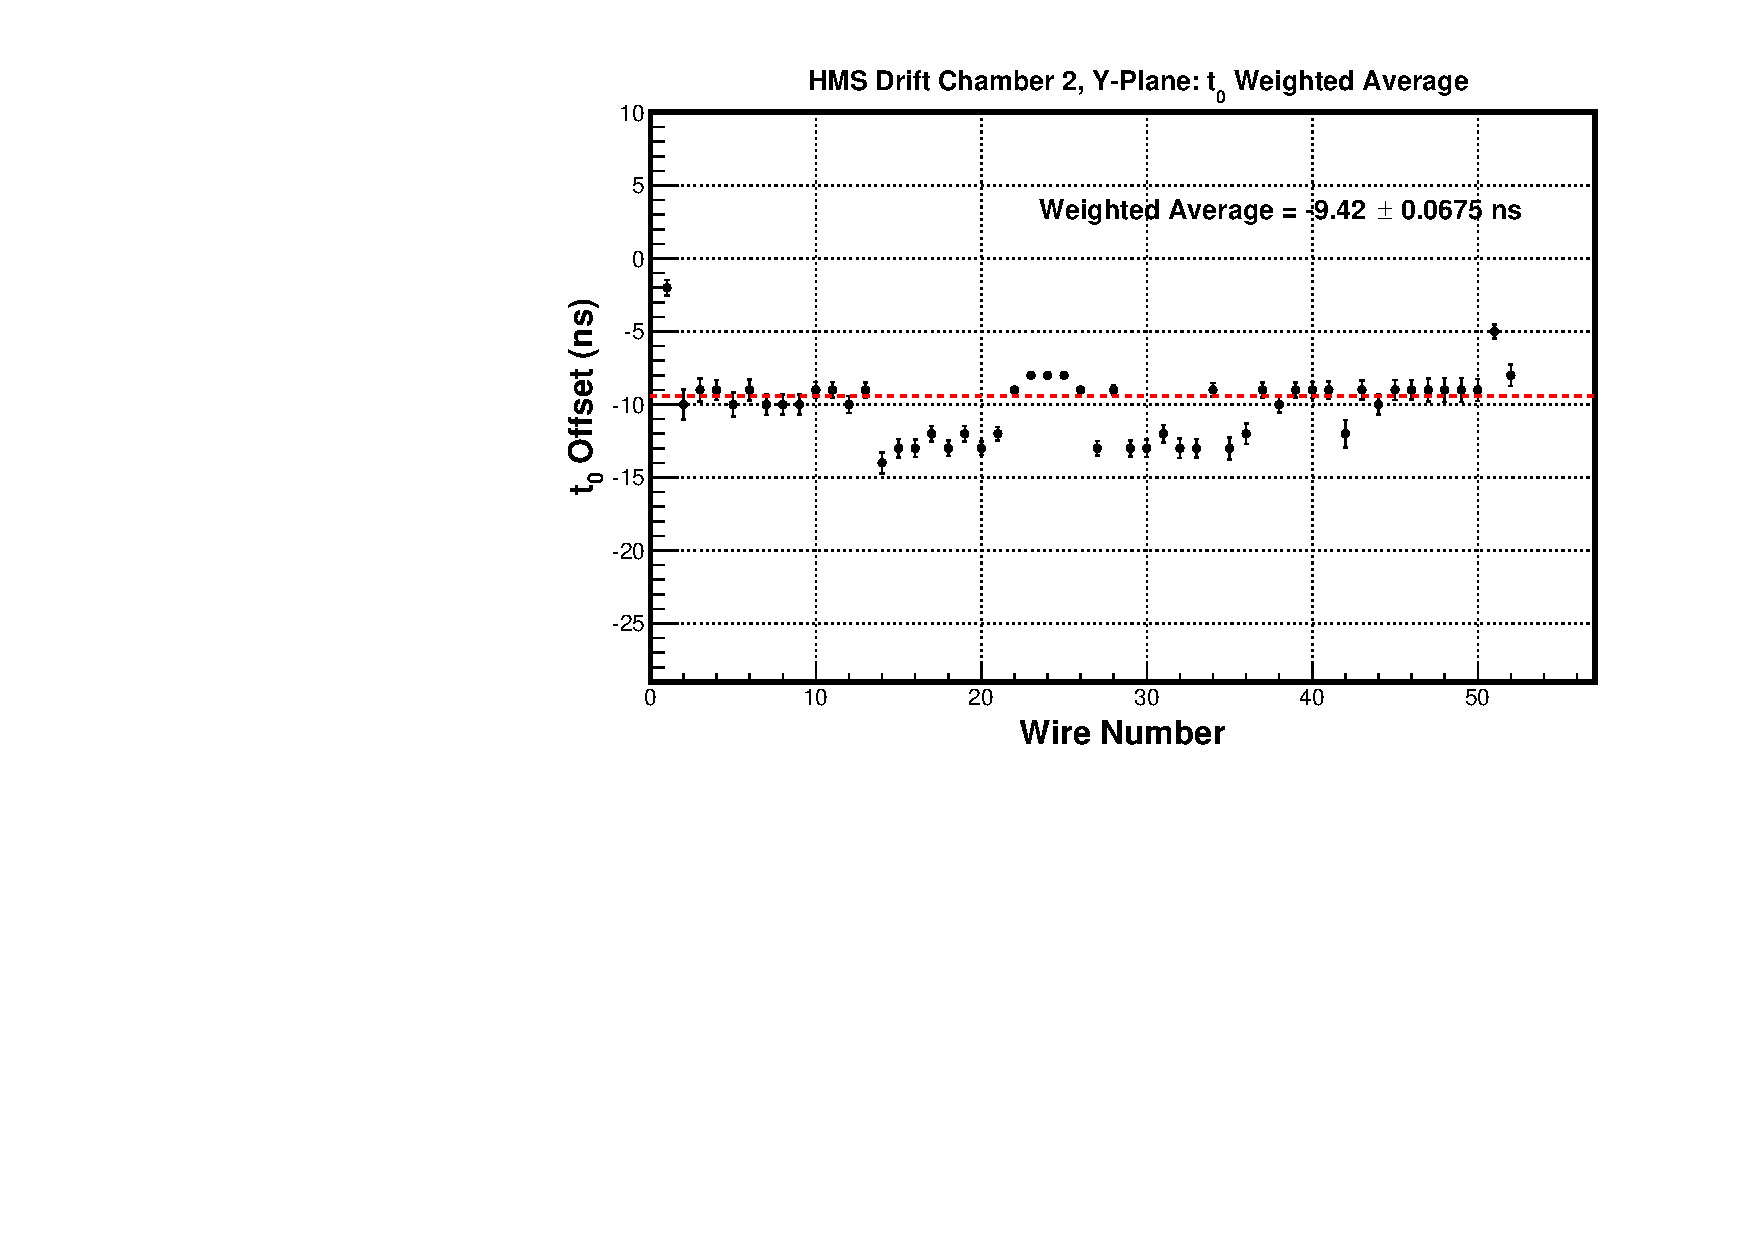
\includegraphics[width=3.8in, height=2.3in]{hdc2y1_wght_avg.pdf}
  \caption{Weighted average of the $``t_{0}"$ offset for all wires in the Y-plane of drift chamber 2.}
  \label{fig:hdc2y1_wght_avg}
\end{figure}\\
The weighted average over all wires is assigned as the $``t_{0}"$ of the plane. When this procedure is done for all planes
in both chambers, the drift times should be aligned at $t_{0}$=0 ns. (See Figure \ref{fig:t0_corr})
\begin{figure}[!ht]
  \centering
  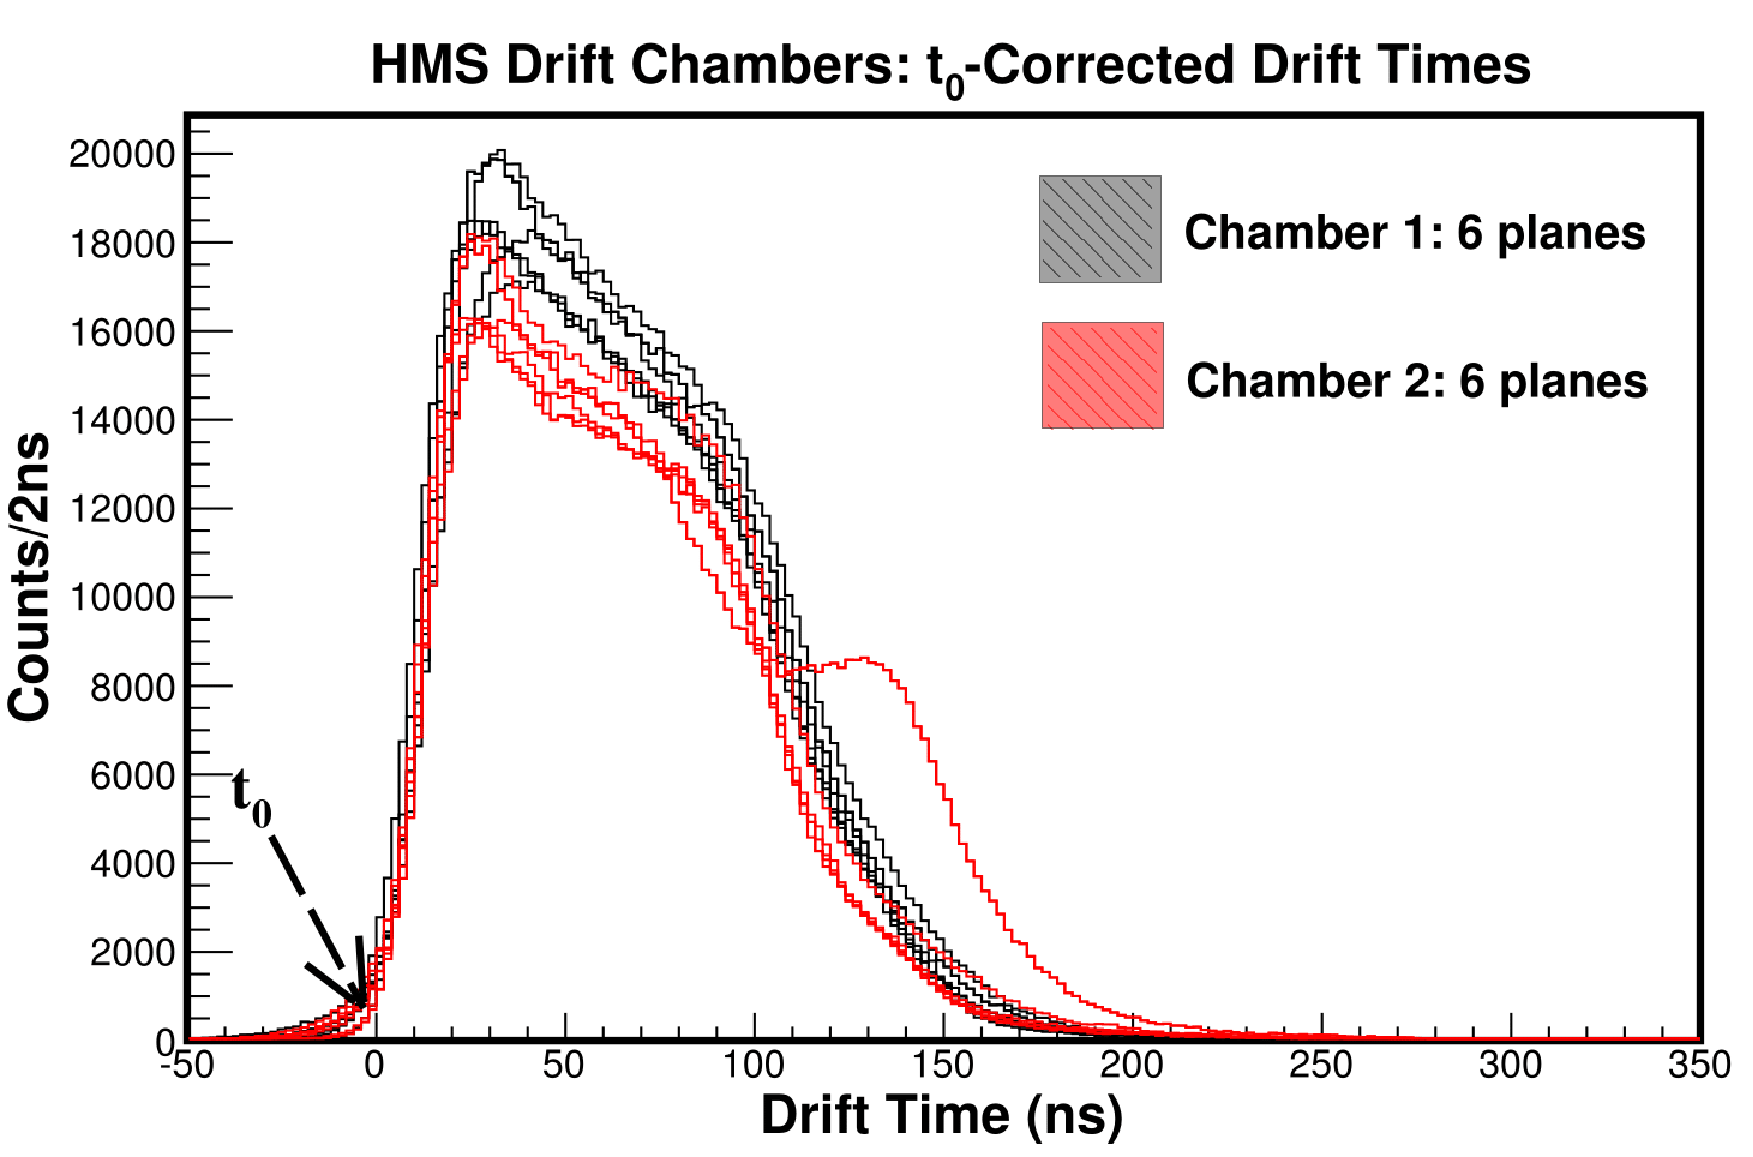
\includegraphics[width=3.6in, height=2.7in]{t0_corr_times.pdf}
  \caption{Corrected drift time spectra for all planes in both drift chambers.}
  \label{fig:t0_corr}
\end{figure}\\
\indent To determine the drift distances from drift time spectra, it is assumed that the
drift distance is uniformly distributed across the cell. This assumption is based on the fact that
a cell is uniformly illuminated with particles, and the ions have an approximately uniform drift velocity
which implies there should be no preferred drift distance for any ionized charge.
Mathematically, the drift distance is calculated as follows,
\begin{equation}\label{eq:2}
d_{drift}(\tau = T) = \frac{\Delta}{2} \frac{\int_{t_{0}}^{T<t_{max}}F(\tau)d\tau}{\int_{t_{0}}^{t_{max}}F(\tau)d\tau}
\end{equation}
where $\Delta$ is the cell width and $F(\tau)$ is the drift time distribution integrated from $t_{0} = 0$ ns to some arbitrary time $T<t_{max}$
where $t_{max}$ is maximum drift time within a cell. The normalization constant in front of the integral is the maximum
drift distance (0.5 cm). In the limiting cases of Eq.\ref{eq:2}, the drift distance becomes
\begin{equation}
  d_{drift} =\begin{cases}
               0 \text{ cm}, & \tau = 0 \text{ ns} \\
               0.5 \text{ cm}, & \tau = t_{max}
            \end{cases}
\end{equation}
which is the expected drift distance at the sense wire ($\tau=0 $ns) and at the edges of the cell ($\tau = t_{max}$). \\
\indent Due to the finite resolution of the TDCs and other factors involved, the drift times are not determined to infinite precision and
the integrals in Eq.\ref{eq:2} become a sum over a finite bin width,
\begin{align*}
\int_{\tau}F(\tau)d\tau \longrightarrow \sum_{bin(\tau)} \underbrace{F(\tau)}_{binContent}\cdot\underbrace{\Delta\tau}_{binWidth}
\end{align*}
Re-writing the ratio of integrals Eq.\ref{eq:2} in terms of the finite sums, one obtains
\begin{equation}\label{eq:4}
\frac{\sum\limits_{bin(t_{0})}^{bin(t_{0}+T)}F(\tau)\Delta\tau}{\sum\limits_{bin(t_{0})}^{bin(t_{0}+t_{max})}F(\tau)\Delta\tau} \rightarrow \boxed{\frac{1}{N_{tot.}}\sum\limits_{bin(t_{0})}^{bin(t_{0}+T)}F(\tau)}
\end{equation}
The ratio in Eq.\ref{eq:4} are the lookup values used to convert drift time to distance for an arbitrary drift time. The
numerator represents the sum of all bin contents up to a drift time $T$, and the denominator represents the sum over the
bin contents of all drift times up to $t_{max} $, in a given plane. The bin width, $\Delta\tau$,
is a constant (2 ns) during the sum, therefore it is cancelled, which simplifies the equation as a ratio of the sum of bin contents (up to some drift time) and
the sum over all bin contents (up to a maximum, $t_{max}$), $N_{tot}$.  \\
\indent The results of this calibration are per plane look-up tables that map any given drift time to a drift distance in
that plane. The drift distance for the Y-plane of drift chamber 2 is shown in Figure \ref{fig:hdc_dist}.
\begin{figure}[!ht]
  \centering
  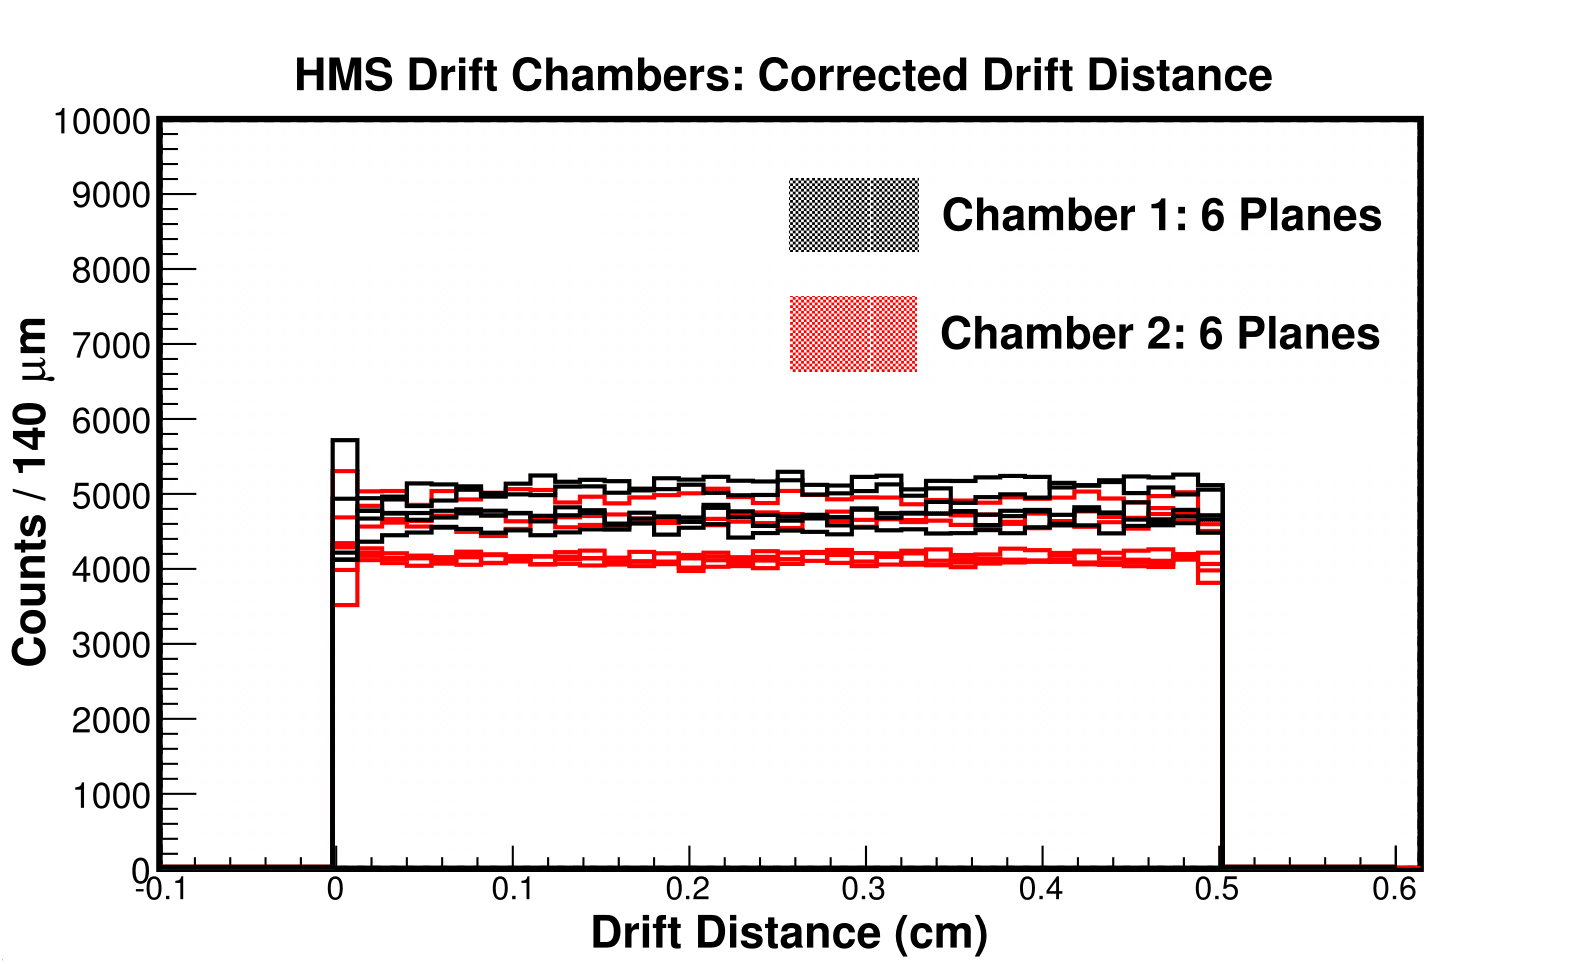
\includegraphics[width=3.6in, height=2.7in]{hdc_distance.png}
  \caption{Corrected drift distance spectra for all planes in both drift chambers.}
  \label{fig:hdc_dist}
\end{figure}
As expected, the drift distances for all planes are uniformly distributed across the cell width. A minor problem
encountered during the calibration procedure was that for some of the calculated drift distances, there was either
a large and small number of counts at the edges (0 or 0.5 cm) whereas in the central region ($\sim$ 0.1-0.3cm), the counts
were uniformly distributed.(See Figure \ref{fig:hdc2y1_uncorr})
\begin{figure}[!ht]
  \centering
  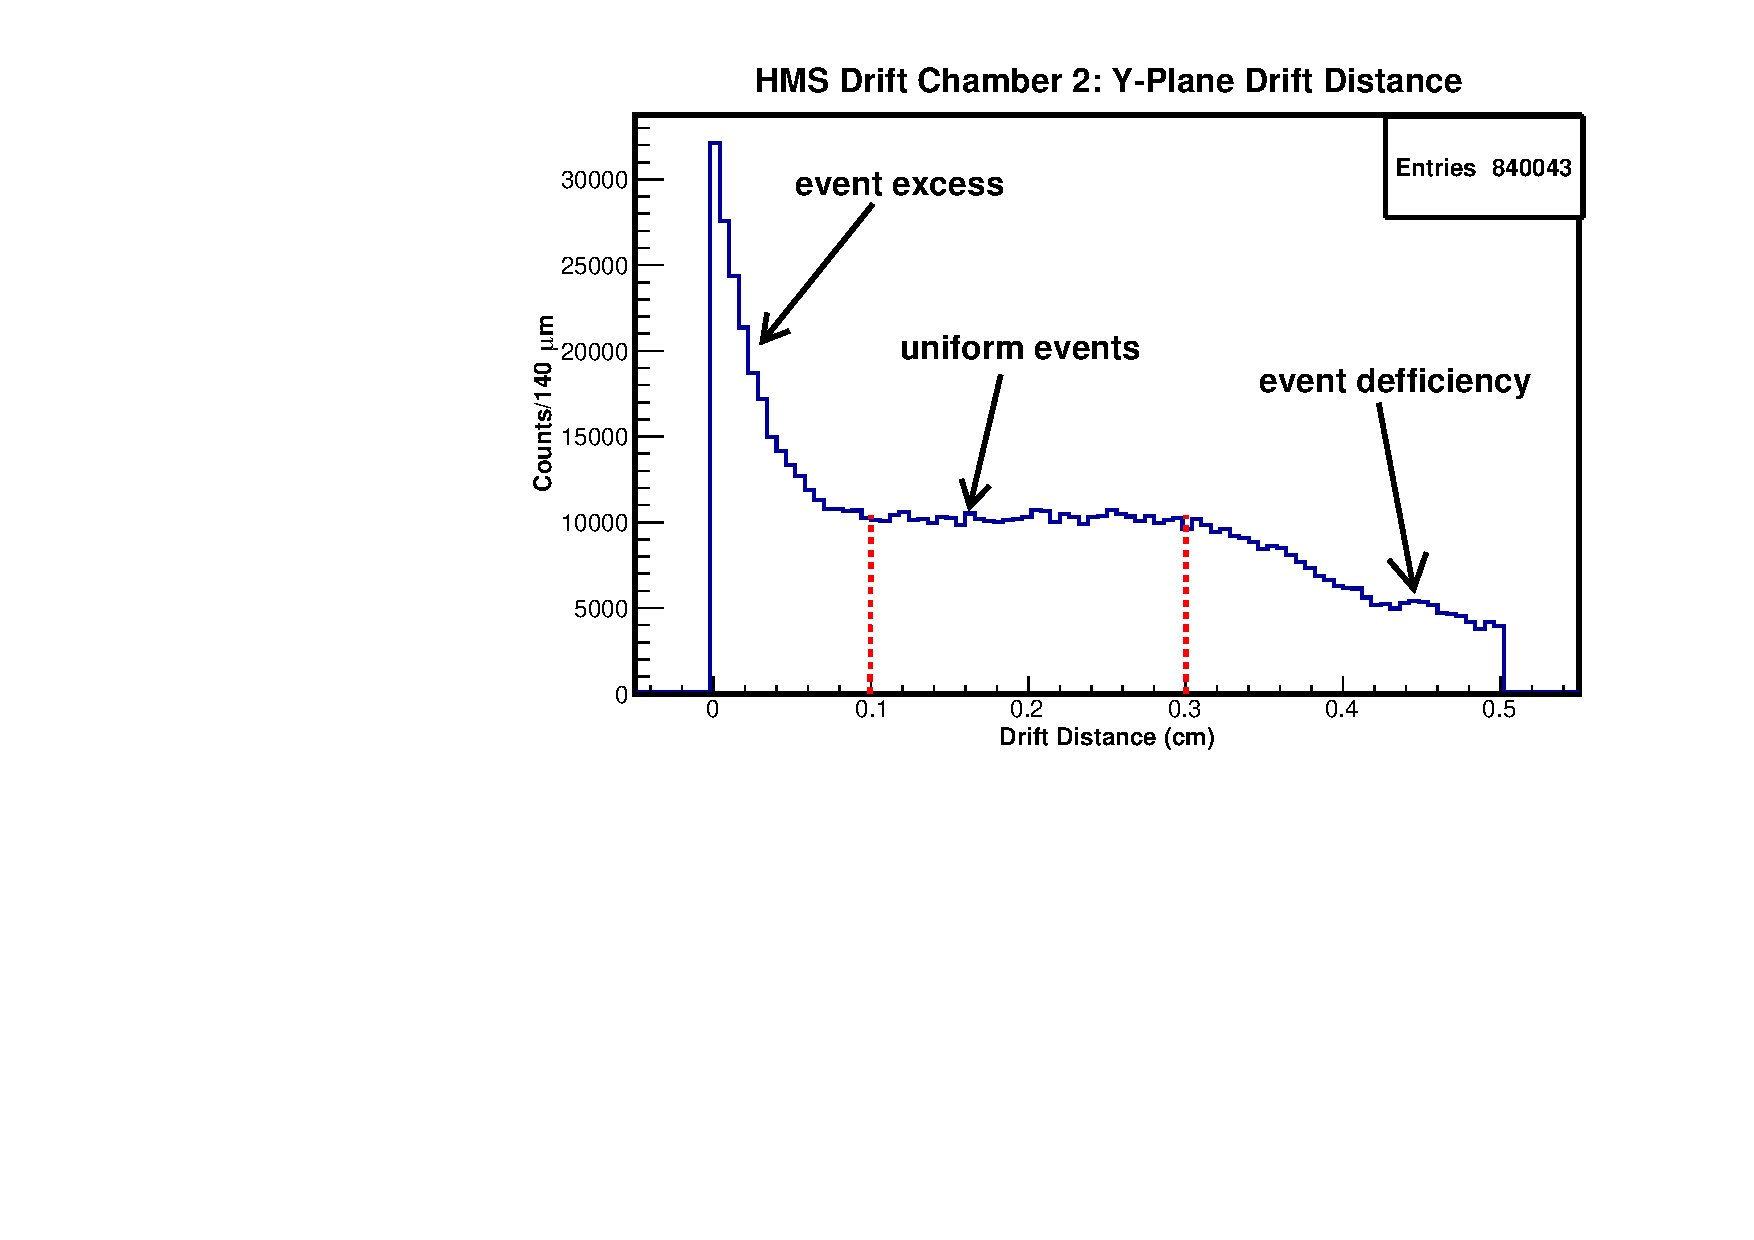
\includegraphics[width=3.6in, height=2.7in]{hdc_2y1_uncorr.pdf}
  \caption{Uncorrected drift distance spectrum.}
  \label{fig:hdc2y1_uncorr}
\end{figure}\\
\indent The weighted $t_{0}$'s determined from calibration had to be manually offset in order to correct
for events accumulating at the edges. This is due to a significant variation ($\sim$ 5-10 ns) in the $t_{0}$'s for groups of wires
in a plane, which affects the weighted average for that plane. To overcome this difficulty, the $t_{0}-$correction
must be applied to individual sense wires rather than taking a weighted average. The procedure to include individual wire
$t_{0}$-offsets is currently in progress.
\section{Drift Velocity Calculation}
Drift velocities of free electrons are sensitive to the gas mixture used in
the chamber as well as the high voltage applied to field wires, as they govern the shape of the electric field that will cause ions to drift. A typical graph
of drift velocities as a function of field strength for various Argon/Ethane mixtures.
mixtures is shown in Figure \ref{fig:drift_vel_vs_Efield}.
\begin{figure}[!ht]
  \centering
  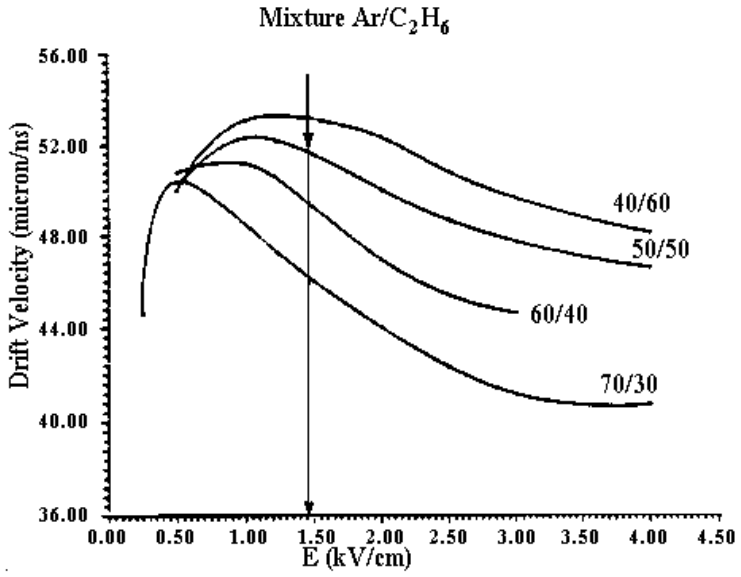
\includegraphics[width=3.2in, height=2.3in]{drift_vel_vs_Efield.png}
  \caption{Drift velocity variation with electric field. Figure courtesy of PHOENIX at Brookhaven National Lab (BNL).}
  \label{fig:drift_vel_vs_Efield}
\end{figure}\\
During the calibration run, the HMS drift chambers operated at a 50:50 mixture by volume of Argon/Ethane. The drift velocities
were determined by taking the ratio of drift distance to drift time per plane. The correlation shows a linear relationship
between distance and time indicating a uniform drift velocity throghout all cells conforming a plane. (See Figure \ref{fig:drift_velocity})
\begin{figure}[!ht]
  \centering
  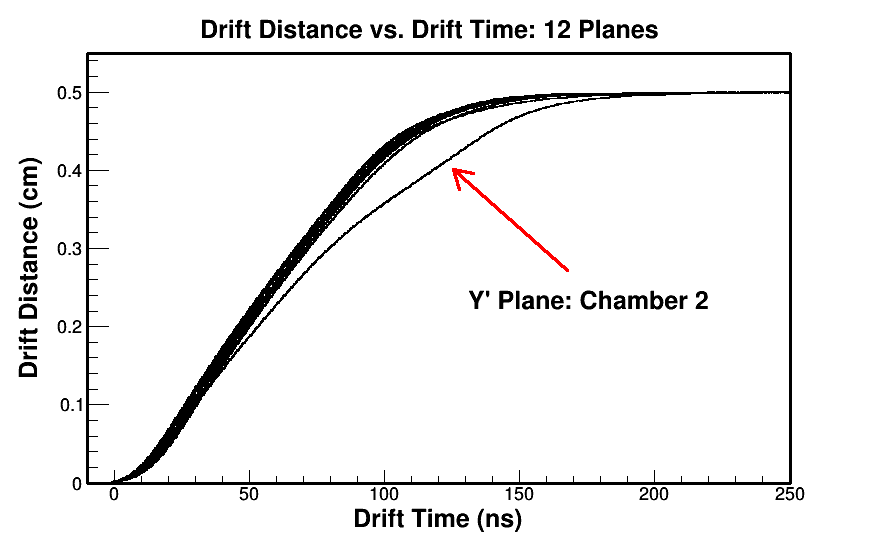
\includegraphics[width=3.6in, height=2.7in]{drift_velocity.png}
  \caption{Correlation between drift distance and drift time for both drift chambers.}
  \label{fig:drift_velocity}
\end{figure}\\
The Y'-plane in chamber 2 shows a significant deviation from the rest. This could indicate a possible variation in the
high voltage applied to the field wires in that plane which leads to variations in the electric field causing variations
in drift velocities. (See Figures \ref{fig:drift_vel_dc1} and \ref{fig:drift_vel_dc2})
\begin{figure}[!ht]
	\centering
	\begin{subfigure}{0.4\textwidth} % width of left subfigure
		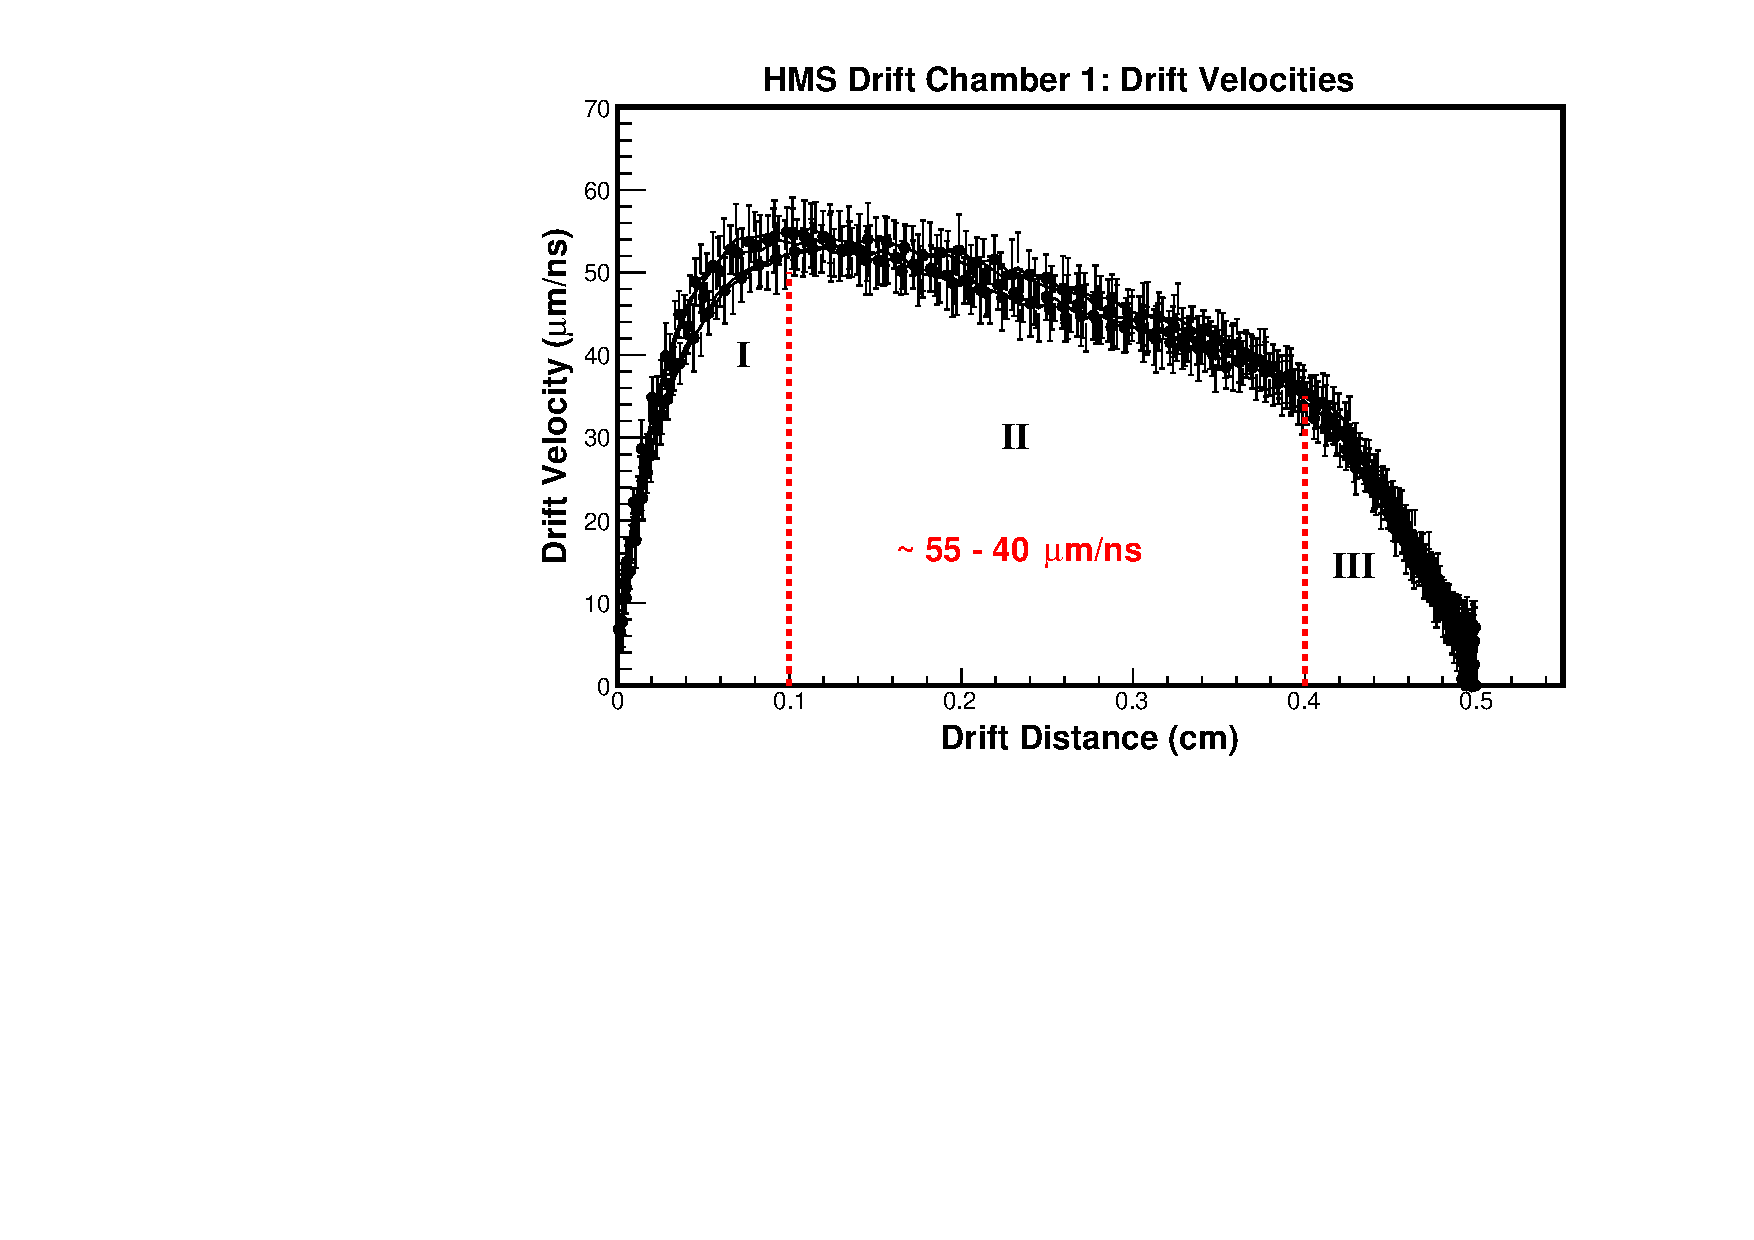
\includegraphics[width=\textwidth]{drift_vel_dc1.pdf}
		\caption{Drift velocity vs. drift distance for all planes in chamber 1.} % subcaption
    \label{fig:drift_vel_dc1}
	\end{subfigure}
	\vspace{1em} % here you can insert horizontal or vertical space
	\begin{subfigure}{0.4\textwidth} % width of right subfigure
		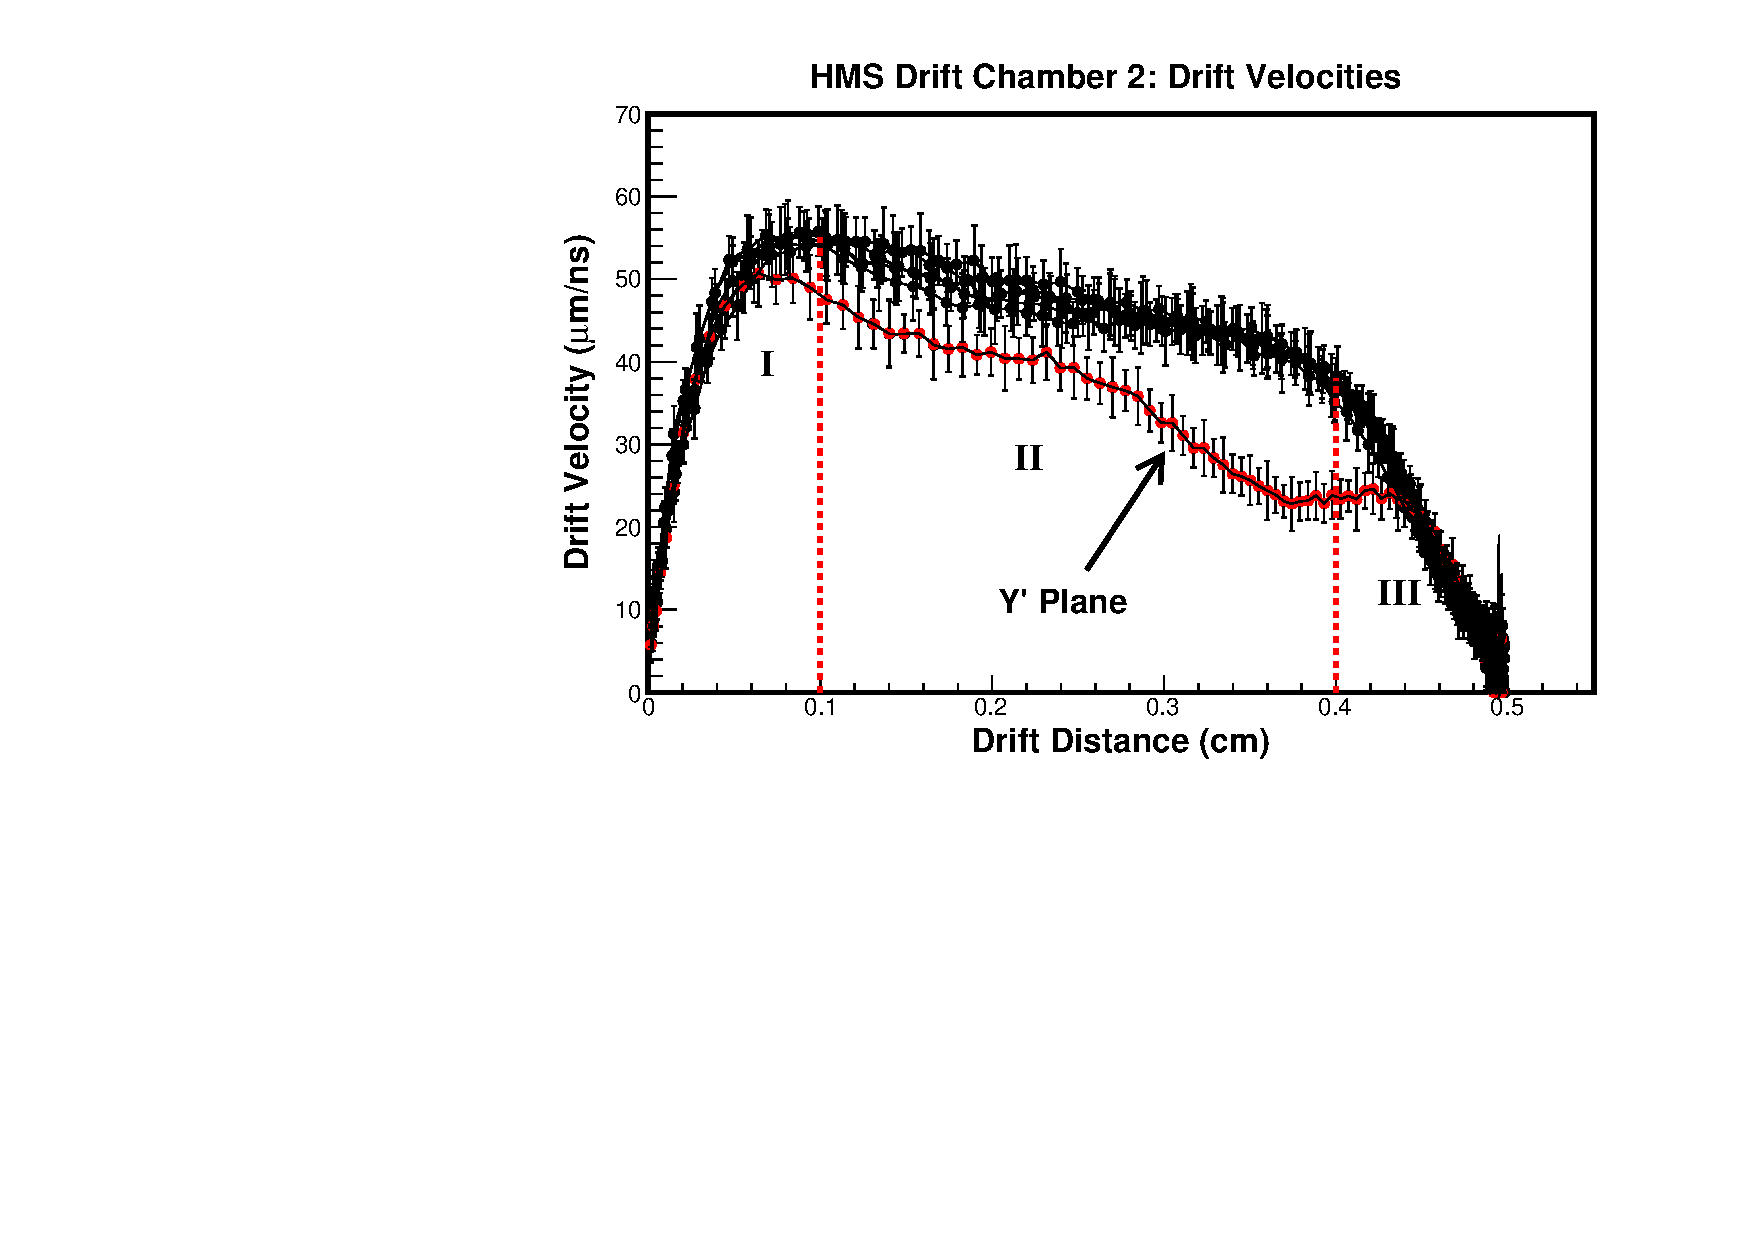
\includegraphics[width=\textwidth]{drift_vel_dc2.pdf}
		\caption{Drift velocity vs. drift distance for all planes in chamber 2.} % subcaption
    \label{fig:drift_vel_dc2}
  \end{subfigure}
	\caption{Drift velocity variation as a function of drift distance for all planes in both chambers.} % caption for whole figure
  \label{fig:drift_vel}
\end{figure}\\
The linear correlation that exists between drift time and distance in Figure \ref{fig:drift_velocity} shows
the drift velocity is mostly constant throughout all planes. The small variations of drift velocity with drift
distance observed in Figure \ref{fig:drift_vel}, however, shows that the drift velocity is not truly a constant,
but varies by a few microns/ns far from the cell edges or center (region II). By performing a linear fit to
the time to distance correlation in steps of 2 ns intervals, the small variations in drift velocity become apparent. The slope
of the linear fit (drift velocity) was plotted versus the drift distance as shown in Figure \ref{fig:drift_vel}.
From Figure \ref{fig:drift_vel}, large variations in the drift velocity can also be observed  at the edges (region III)
and center (region I) of a cell. This effect is due to the non-uniformity of the electric field in these regions.

\section{Drift Chamber Efficiencies and Residuals}
The per plane efficciencies were determined for all planes. The efficinecy of any given plane
in a chamber is defined as the ratio of the number of hits that were detected by the plane to the number of hits that
\textit{should} have been detected by that plane.
Where a \textit{hit} is defined as a detectable signal in the chamber from ionized charges produced by the passage of a
particle. Mathematically, the efficiency of the $i^{th}$ plane is given by \\
\begin{equation*}
\epsilon_{i} = \frac{\# \text{ hits that were detected by the $i^{th}$ plane}}{\# \text{ hits that \textit{should} have been detected by the $i^{th}$ plane}}
\end{equation*}
with the condition that the hit was also detected by the remaining five planes in the chamber. The
efficiencies of both chambers are summarized in Table \ref{tab:eff}.
\begin{table}[!h]
  \scalebox{0.8} {
\begin{tabular}{ |l|l|l| }
\hline
\multicolumn{3}{ |c| }{\textbf{HMS Drift Chamber Efficiencies}} \\
\hline
\textbf{Plane} & \textbf{Chamber 1} (\%) & \textbf{Chamber 2} (\%) \\ \hline
\multirow{6}{*}{}
X  & 95.8 & 99.4  \\ \hline
Y  & 98.7 & 99.7  \\ \hline
U  & 97.7 & 96.6  \\ \hline
V  & 96.5 & 97.7  \\ \hline
Y' & 99.0 & 97.7  \\ \hline
X' & 94.9 & 97.2  \\ \hline
\end{tabular}
}
\caption{Drift chamber plane efficiencies}
\label{tab:eff}
\end{table}\\
\indent The best way to determine the drift chamber performance is by measuring the spatial resolution, or how
well it can measure the position of particle tracks. This measurement is done through the determination of per plane
residuals. For a particle traversing at least 4 planes of the chamber, a collection of space-points (X,Y) is measured based on the
wires that fired. The space points are fitted with a straight line such as to minimize the chi-square, and obtain a best
fit. The line fit is then compared to the meausured space-point from the plane wires that fired, and the difference is called the \textit{residual}
for that plane. The residuals are calculated on an event by event basis, and should be centered around zero. (See Figure \ref{fig:hdc1y1_residual})
\begin{figure}[!ht]
  \centering
  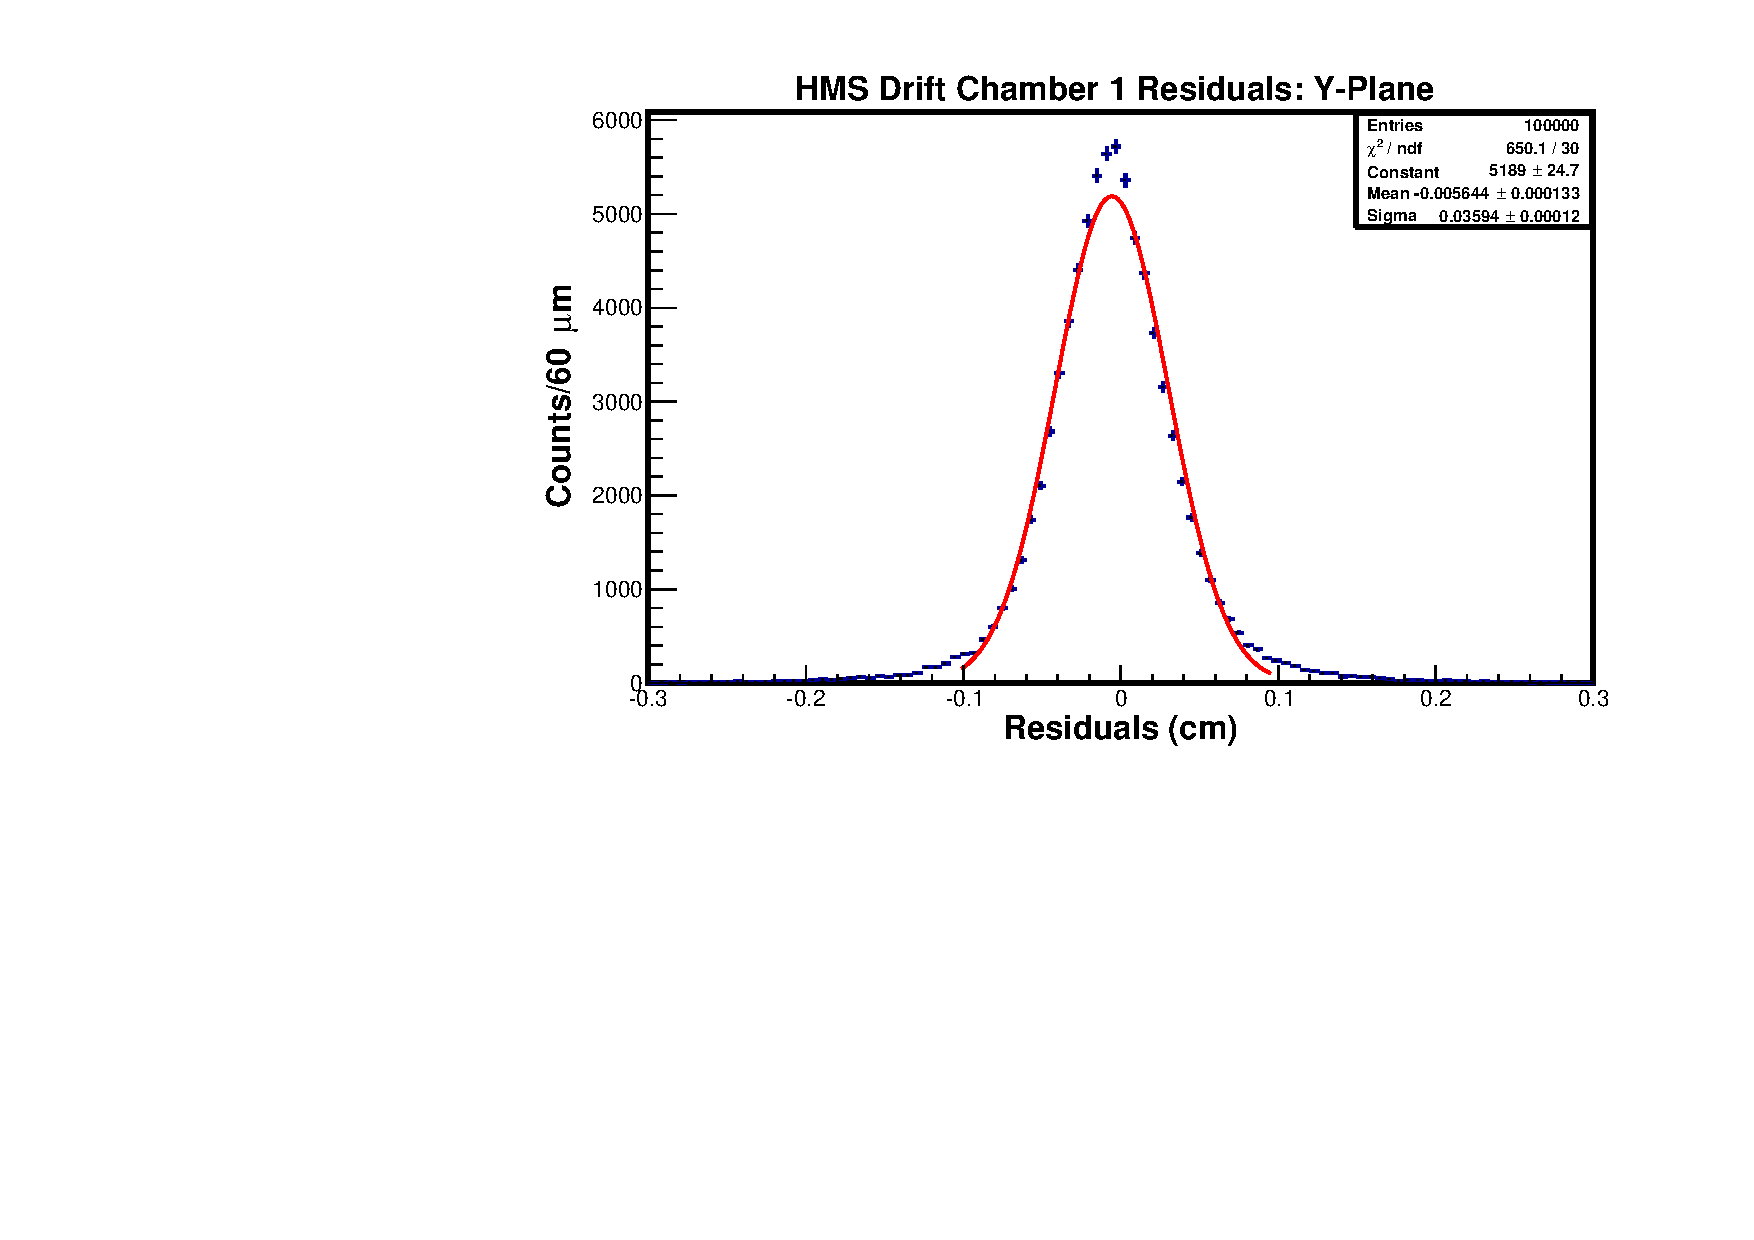
\includegraphics[width=3.6in, height=2.7in]{hdc1y1_residuals.pdf}
  \caption{Residuals for the Y-plane in chamber 1. The Full Width at Half Maximum (FWHM or $\sigma$)  is representative the
  spatial resolution.}
  \label{fig:hdc1y1_residual}
\end{figure}\\
A gaussian fit was done for all planes in both chambers to extract the space resolution of the chambers. The fit results are
summarized in Table \ref{tab:res}
\begin{table}[!h]
\scalebox{0.8} {
\begin{tabular}{ |l|l|l| }
\hline
\multicolumn{3}{ |c| }{\textbf{HMS Drift Chamber Residuals}} \\
\hline
\textbf{Plane} & \textbf{Chamber 1}, $\sigma(\mu m)$ & \textbf{Chamber 2}, $\sigma(\mu m)$ \\ \hline
\multirow{6}{*}{}
X & 416$\pm$1.69 & 388$\pm$1.60 \\ \hline
Y & 360$\pm$1.18 & 408$\pm$1.22 \\ \hline
U & 361$\pm$1.29 & 327$\pm$1.27 \\ \hline
V & 382$\pm$1.47 & 323$\pm$1.28 \\ \hline
Y'& 383$\pm$1.31 & 391$\pm$1.16 \\ \hline
X'& 419$\pm$1.63 & 384$\pm$1.55 \\ \hline
\end{tabular}
}
\caption{Drift chamber plane residuals}
\label{tab:res}
\end{table}

\section{Summary}
This report has outlined the steps taken to calibrate the HMS drift chambers using data taken on March 2017. The outline
also covered some of the difficulties encountered in the calibration procedure, and the steps taken to overcome them. The effects
of the gas mixture and applied high voltage on the drift velocities was also briefly discussed. Finally, two
performance criterions (efficiencies and residuals) used to describe the performance of the drift chambers were investigated. The
efficiencies described how well were the chambers able to detect hits produced by the passage of a particle. The residuals described
how well does the measured particle position in each plane compare to the best track fit through all six planes in each chamber.

%\clearpage
\bibliography{report}
\bibliographystyle{acm}

% Your document ends here!
\end{document}
